\subsubsection{Momento generado por un humano}

La fuerza nominal $F_n$ que puede generar el brazo de un humano es de \cite{Biomec}:

\begin{center}
    $F_n = 8.5 \frac{kg}{cm^2}$
\end{center}

Considerando la longitud estándar de un brazo humano, se puede generar un momento $M_c$ de \cite{Biomec}:

\begin{center}
    $M_c = 66.7 Nm$
\end{center}

Al considerar la anchura del compostador, se tiene que el brazo de palanca $L$ más grande posible es:

\begin{center}
    $L = 0.3 m$
\end{center}

Por lo que la fuerza máxima queda definida por:

\begin{center}
    $F_{max} = \frac{M_c}{F_n}=\frac{66.7}{0.3} = 222.33 N$ \\
    $F_{max} \approx 222.5 N $
\end{center}

Esta fuerza es suficiente sabiendo que no se trituraran huesos, y la materia orgánica más dura a moler serán cascaras de sandía.

Sabiendo todo esto, se procedió a buscar una solución en el mercado que se adaptara a las necesidades del proyecto. 

Después de una amplia búsqueda, se determinó que un molino manual de carne se adaptaba de manera correcta al proyecto.

El molino seleccionado cumple con la capacidad de trituración que se busca tener, este triturador, (figura \ref{fg:molino}), es capaz de procesar hasta 82 kilogramos de carne por hora.

\begin{figure}[h!]
            \centering
            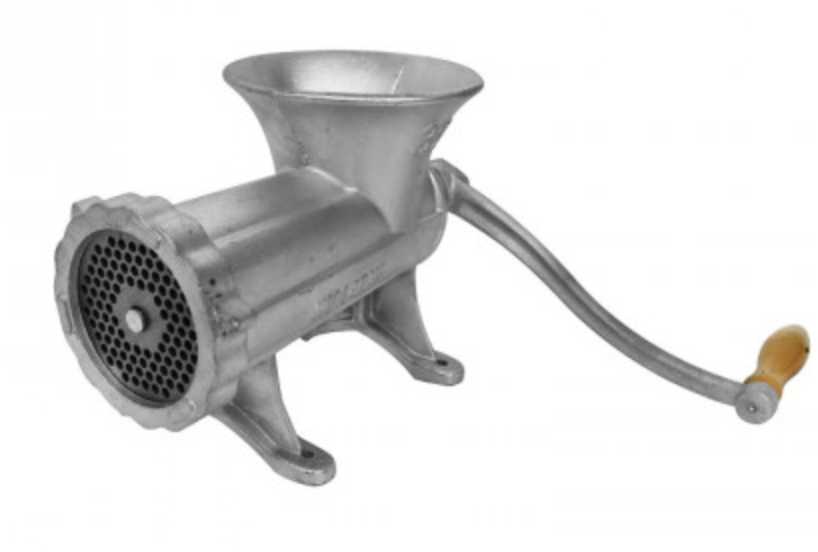
\includegraphics[scale=0.8]{images/Capitulo 4/S4/Molino 32.png}
            \caption{Molino de carne manual}
            \label{fg:molino}
\end{figure}


